  \documentclass[crop,tikz]{standalone}% 'crop' is the default for v1.0, before it was 'preview'
%\usetikzlibrary{...}% tikz package already loaded by 'tikz' option
\usepackage[utf8]{inputenc}

\usepackage{tikz}
\usetikzlibrary{
  arrows,
automata,
backgrounds,
calc,
decorations.pathreplacing,
fit,
petri,
positioning,
shadows,
shapes,
snakes,
}


\begin{document}

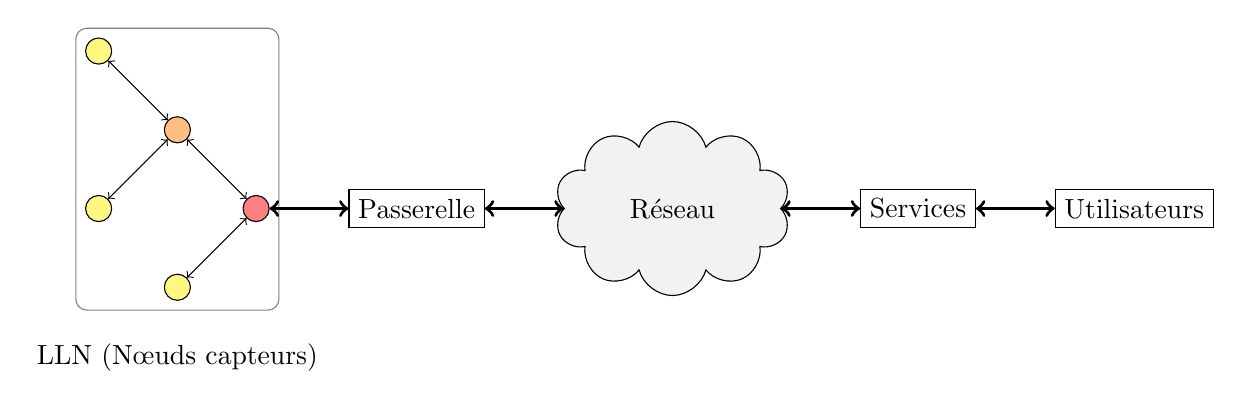
\begin{tikzpicture}

% définition des styles
\tikzstyle{visible}=[draw, fill=blue!50]
\tikzstyle{hidden}=[ draw, fill=gray!20]
\tikzstyle{router}=[circle, draw, fill=orange!50,text=black]
\tikzstyle{child}=[circle, draw, fill=yellow!50,text=black]
\tikzstyle{root}=[circle, draw, fill=red!50,text=black]



% Réseau contraint
\node[root] (LBR) at (-4, 0) {};
\node[router] (2) at (-5, 1) {};
\node[child] (3) at (-5, -1) {};
\node[child] (4) at (-6, 2) {};
\node[child] (5) at (-6, 0) {};

% les nœuds
\node[draw, right=of LBR] (gw) {Passerelle};


% \node[cloud, cloud puffs = 10, minimum width = 4cm, draw, fill = gray!10] (cloud) at (5,0) {Réseau local};
\node[draw, cloud, cloud puffs = 10, minimum width = 3cm, draw, fill = gray!10, right=of gw] (cloud) {Réseau};
\node[draw, right=of cloud,] (service) {Services};
\node[draw, right=of service] (users) {Utilisateurs};  


\node [fit=(LBR) (2) (3) (4) (5), rounded corners, draw=black!50] (lln) {};
\node [below=.3 cm of lln] {LLN (Nœuds capteurs)};

\path

% Réseau contraint
(gw.west) edge[<->, very thick]  (LBR) 
% (gw.west) edge[->, thick, bend right=20]  (LBR) 
(LBR) edge[<->] (2)
(LBR) edge[<->] (3)
(2) edge[<->] (4)
(2) edge[<->] (5)

% Réseau conventionnel
(gw.east) edge[<->, very thick,] (cloud.west)
(cloud.east) edge[<->, very thick] (service.west)
(service.east) edge[<->, very thick] (users.west)

;

\end{tikzpicture}
\end{document}